%!TEX root = ../lectures_olympics.tex

\chapter{振动和波}
振动和波动是自然界当中广泛存在的两类现象。
有些振动现象非常容易观察,例如系在弹簧上的物体的往复运动,或者系在绳子一端的球在重力作用下的摆动;有些振动则不太容易被查觉,例如用力敲击桌子以后它实际在作微小的振动,用一些手段可以展示这类振动;还有的振动现象靠肉眼根本不可能看到,必须依靠精密的仪器,例如分子的振动。
各种各样的振动现象的一个共同特点就是一些物理在某一给定值周围随时间做\emph{往复变化},有的振动十分规则,例如由弹簧连接的物体,有的振动则不太那么规则,例如通过地震仪探测到的地球振动的信号,就像图\ref{fig: ow-简单和复杂的振动}中所展示的那样。
当一个物体在作振动时,很有可能通过直接互间接的相互作用引起它周围物体的振动,那些被影响了的物体又会引起更远处物体的振动,这样一个物体的振动效果看上去就被传递了出去,这类现现统称为\emph{波}。
自然界中几乎所有的能量传递过程其背后都是波动现象。
水波很容易产生的观察,声波则需要借助一些工具才能够展示出来,太阳的能量依靠电磁波传向地球,2016年春节前后人们又通过长期不懈的观测发现了引力波。
这里我们就来学习支配这些振动和波动现象背后的物理定律。
\begin{figure}[hbtp]

\centering
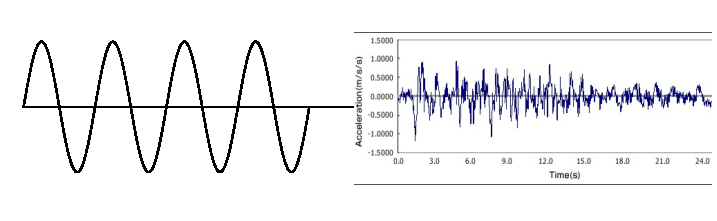
\includegraphics[width=0.7\textwidth]{images/ow-oscillation-examples.pdf}
\caption{振动是某一物理量在某点附近往复变化,左图:弹簧振子,右图:地震波}\label{fig: ow-简单和复杂的振动}
\end{figure}

\section{简谐振动}
我们首先来学习图\ref{fig: ow-简单和复杂的振动}左边那种简单的振动过程,像右图所示的复杂振动过程可以看作是多个简单的振动的叠加。
如果一个振动质点在坐标系中的位置随时间的变化关系由时间的正弦或余弦函数所给出,就称该物体在作\emph{简谐振动}。
用$x(t)$表示作简谐振动质点的位置,它随时间的关系由
\begin{equation}\label{eqn: ow-简谐振动x-t}
x(t) = A\cos(\omega t+\varphi)
\end{equation}
式中$A$称做简谐振动的\emph{振幅},$\omega$为简谐振动的\emph{角频率},$\varphi$则是简谐振动的\emph{相位}。
当它们三个物理量均为已知时,我们就掌握了一个做简谐振动质点的全部信息,振幅、角频率和相位一起称做简谐振动的三要素。
除了它们三个以外,还有两个相关的物理量,一个是简谐振动的周期,它由角频率所决定,和圆周运动类似
\begin{equation}
T = \frac{2\pi}{\omega}
\end{equation}
它用来描写完成一个完整的周期运动所需要的时间,另外一个是简谐振动的频率
\begin{equation}
f = \frac{1}{T}
\end{equation}
用来表达单位时间里能够完成周期运动的次数。

当一个做简谐振动质点的位置随时间的关系\ref{eqn: ow-简谐振动x-t}被给定了以后,它的其它物理量随时间的变化关系可由位置随时间的关系而导出。
例如振动质点的速度就是位置随时间的导数:
\begin{equation}\label{eqn: ow-简谐振动v-t}
v(t)=\frac{dx}{dt} = -\omega A\sin(\omega t+\varphi)
\end{equation}
类似地,加速度就是速度对时间的导数:
\begin{equation}\label{eqn: ow-简谐振动a-t}
a(t) = \frac{dv}{dt}=\frac{d^2x}{dt^2} = -\omega^2 A\cos(\omega t+\varphi) =-\omega^2 x(t)
\end{equation}




\begin{example}
除了用式\ref{eqn: ow-简谐振动x-t}表示一个简谐振动以外,为了避免使用相位另外一种等效的方法为
\[
x(t)=a\cos\omega  t+b\sin\omega t
\]
试给出$a、b$与式\ref{eqn: ow-简谐振动x-t}中的振幅和相位$A、\varphi$之间的代数关系。
\tagged{student}{\vspace*{4cm}}
\begin{taggedblock}{teacher}
\newline
解析:利用三角函数之间的关系我们有
\[x=A[\cos\omega t\cos\varphi -\sin\omega t\sin\varphi ]\]
与新的表达式做比较可得
\[
a = A\cos\varphi,\qquad b =- A\sin\varphi
\]
反过来则是
\[
A = \sqrt{a^2+b^2},\qquad \varphi =- \arctan\frac{b}{a}
\]
\end{taggedblock}
\end{example}


从牛顿运动定律可知,任何物体运动状态的变化都是由外力作用引起的,做简谐振动的质点也不例外。
根据质点的加速度的表达式\ref{eqn: ow-简谐振动a-t}可知,当振动质点的质量为$m$时,它所受到的合外力则是
\begin{equation}\label{eqn: ow-回复力与频率的关系}
F=ma = -m\omega^2 x.
\end{equation}
也就是说,当一个质点所受合外力正比于它偏离平衡位置$x=0$的距离$x$并且无论所处位置如何均指向平衡位置时,质点将做简谐振动!
满足这样条件的外力统称为简谐振动的\emph{回复力}。

产生回复力的种类有很多,这其中最简单的回复力自然就是满足胡克定律的弹簧。
如图所示,在光滑的水平表面上有一个劲度系数为$k$的弹簧,其平衡位置为$O$点,它的一端固定,另一端自由并且与一个质量为$m$的质点连接。
建立以弹簧平衡位置为原点的坐标系,当质点的位置为$x$时它所受到的弹性力
\begin{equation}
F=-kx
\end{equation}
可见此时弹簧弹性力满足回复力的条件,质点将做简谐振动。
与回复力的表达式\ref{eqn: ow-回复力与频率的关系}相比较可知弹簧弹性系数$k$,质点质量$m$与简谐振动角频率之间满足关系
\begin{equation}
k=m\omega^2\qquad \textbf{或}\qquad \omega=\sqrt{\frac{k}{m}},
\end{equation}
这时简谐振动的周期可以写为
\begin{equation}
T = 2\pi\sqrt{\frac{m}{k}},
\end{equation}
可以看到简谐振动的周期由弹性系数和振动质点的质量共同决定。

\begin{example}
将两根原长相同,劲度系数分别为$k_1$和$k_2$的弹簧。
求它们并联或串联时连接一个质量为$m$的质点做简谐振动的角频率和周期。
\tagged{student}{\vspace*{4cm}}
\begin{taggedblock}{teacher}
\newline
解析:两弹簧并联时等效的弹性系数$k=k_1+k_2$,这时振动的角频率和周期分别为
\[
\omega = \sqrt{\frac{k_1+k_2}{m}},\qquad T = 2\pi\sqrt{\frac{m}{k_1+k_2}}
\]
串联时等效弹性系数$k = \frac{k_1k_2}{k_1+k_2}$,这时振动的角频率则是
\[
\omega = \sqrt{\frac{k_1k_2}{(k_1+k_2)m}},\qquad T = 2\pi \sqrt{\frac{m(k_1+k_2)}{k_1k_2}}
\]
\end{taggedblock}
\end{example}

\begin{example}
的一个质量为$m$的重物挂在一个竖直的弹性系数为$k$的弹簧上,求其在平衡位置附近振动的周期。
\tagged{student}{\vspace*{4cm}}
\begin{taggedblock}{teacher}
\newline
解析:$T=2\pi\sqrt{\frac{m}{k}}$
\end{taggedblock}
\end{example}


\begin{example}
判断以下运动是否为简谐振动:

(a)边长为$L$,密度为$\rho$的物体漂浮在密度为$\rho_0>\rho$的液体当中受到竖直方向的扰动。

(b)质量为$M$,半径为$R$的密度均匀球体内部任意一条连接表面两点间通道中物体的运动

(c)劲度系数为$k$的弹簧端点处系有质量为$M$的物体在摩擦系数为$\mu$的水平面上运动。


\tagged{student}{\vspace*{4cm}}
\begin{taggedblock}{teacher}
\noindent
解析:都是
\end{taggedblock}
\end{example}



在弹性力作用下简谐振动质点的机械能包含有它的动能和弹性势能,这样总能量为
\begin{eqnarray}
E& =& \frac{1}{2}mv^2+\frac{1}{2}kx^2\nonumber\\
 &=& \frac{1}{2}m\omega^2A^2\cos^2(\omega t+\varphi)+\frac{1}{2}kA^2\sin^2(\omega t+\varphi)\nonumber\\
 &=&\frac{1}{2}kA^2 = \frac{1}{2}m\omega^2A^2
\end{eqnarray}
能够看到总能量与振幅有着直接的关系,振动物体的总能量为振幅的平方,可以利用振动最远端的弹性势能或当运动到平衡位置的速度来衡量简谐振动的能量。


\begin{example}
竖直悬挂的原长为$l_0$,劲度系数为$k$的轻弹簧一端系为质量为$M$的物体,开始时弹簧处于原长,重物具有向上的速度$v_0$。
证明物体此后的运动为简谐振动并求出振动的平衡位置、振幅、周期。
\tagged{student}{\vspace*{4cm}}
\begin{taggedblock}{teacher}
\newline
解析:平衡位置在弹簧伸长$\frac{Mg}{k}$处,周期$2\pi\sqrt{\frac{M}{k}}$,振幅:$\sqrt{(\frac{Mg}{k})^2+\frac{m}{k}v_0^2}$
\end{taggedblock}
\end{example}

除了角频率和振幅,在有些问题中简谐振动的相位也起着至关重要的作用。
前面已经看到,振动的角频率或周期取决于振动物体和回复力的性质,而振幅则由振动系统的总能量所决定,而相位取决于振动物体的初始状态,一般来说振动物体在$t=0$时的位置和速度。
设$t=0$时振动处于初始位置位置$x_0$、初速度$v_0$的状态,根据简谐振动的运动方程可知它的初始条件与振动的参数之间有关系:
\[
x_0 = A\cos\varphi,\qquad v_0 = -\omega A\sin\varphi
\]
联立以上两式可以解出振动的振幅和相位与初始条件之间满足关系式
\begin{equation}
A = \sqrt{x_0^2+\frac{v_0^2}{\omega^2}},\qquad \varphi = -\arctan\frac{v_0}{\omega x_0}.
\end{equation}
在决定振动的相位时有一定任意性,任何与$\varphi$相差$2\pi$的整数倍的角度能够给出完全相同的振动,一般来说我们将相位取在0到$2\pi$之间,但是请注意这一点并不是必需的。

%\begin{example}
%数字计算相位
%\tagged{student}{\vspace*{4cm}}
%\begin{taggedblock}{teacher}
%\noindent
%解析:
%\end{taggedblock}
%\end{example}
%
%\begin{example}
%代数方法决定相位
%\tagged{student}{\vspace*{4cm}}
%\begin{taggedblock}{teacher}
%\noindent
%解析:
%\end{taggedblock}
%\end{example}



\begin{example}
光滑平面上两个质量均为$m=1\unit{kg}$的质点$A$、$B$由一根原长为$l=2\unit{m}$劲度系数为$k=1\unit{N/m}$的弹簧相连接。
已知$t=0$时两个质点的位置和速度分别为
\[x_A = 0,\qquad x_B = 4,\qquad v_A = 2\unit{m/s},\qquad v_B=0\]
求此后两个质点的位置随时间的关系$x_A(t)$、$x_B(t)$?
\tagged{student}{\vspace*{3cm}}
\begin{taggedblock}{teacher}
\newline
解析:A:$t+1+\sqrt{2}\sin(t-\frac{\pi}{4})$
\\B:$t+3-\sqrt{2}\sin(t-\frac{\pi}{4})$
\end{taggedblock}
\end{example}

\subsection{单摆}
\begin{figure}[hbtp]
\centering
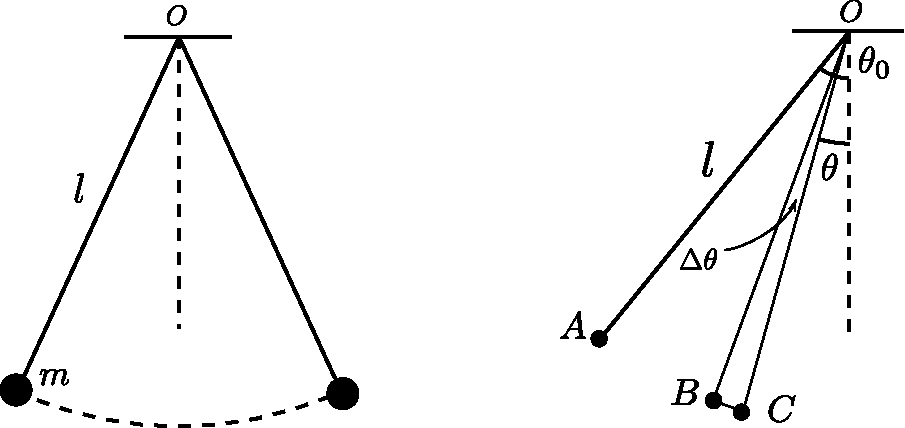
\includegraphics[width=0.6\textwidth]{images/ow-pendulum.pdf}
\caption{悬挂物体的摆动称为单摆,右图为最大摆角为$\theta_0$时的情况}\label{fig: ow-单摆}
\end{figure}
另外一个经典的振动现象来自于自由悬挂的质点,如图\ref{fig: ow-单摆}所示的一根长度为$l$的不可伸长质量忽略不计的细绳一端系于固定点$O$,另一端上系有一个质量为$m$的质点。
当把质点从最低点拉开一个角度后释放,它将围绕最低点往复运动,这个系统称为一个单摆。
我们用摆线与垂线的夹角$\theta$来表示摆球的位置,当物体摆动到最高点时夹角为$\theta_0$,称作单摆的振幅。
单摆的周期与振幅有关,如图\ref{fig: ow-单摆}右图所示,当从最高点$A$下落到由$\theta$角表示的位置$B$时,根据机械能守恒摆球的速度为
\begin{equation}
v = \sqrt{2gl(\cos\theta-\cos\theta_0)}
\end{equation}
从$B$到$C$夹角的变化量记作$\Delta \theta$,这样$BC$的弧长则是$l\Delta \theta$,从$B$摆到$C$所需要的时间
\begin{equation}
\Delta t = \frac{l\Delta\theta}{v}
\end{equation}
取$\Delta\theta\rightarrow 0$的极限并积分,根据运动的对称性可知单摆的周期与振幅的关系为
\begin{equation}
T(\theta_0)= 4\int_0^{\theta_0}\sqrt{\frac{l}{2g}}\frac{d\theta}{\sqrt{\cos\theta-\cos\theta_0}}
\end{equation}
这个函数相当复杂,利用计算机可以作出周期与振幅的图像,从图\ref{fig: ow-单摆的周期和振幅的关系}中可以很清楚地看出当振幅很小时单摆的周期近似地与振幅无关,随着振幅的增加到一定程度以后周期的变化也会增加。

\begin{figure}[hbtp]
\centering
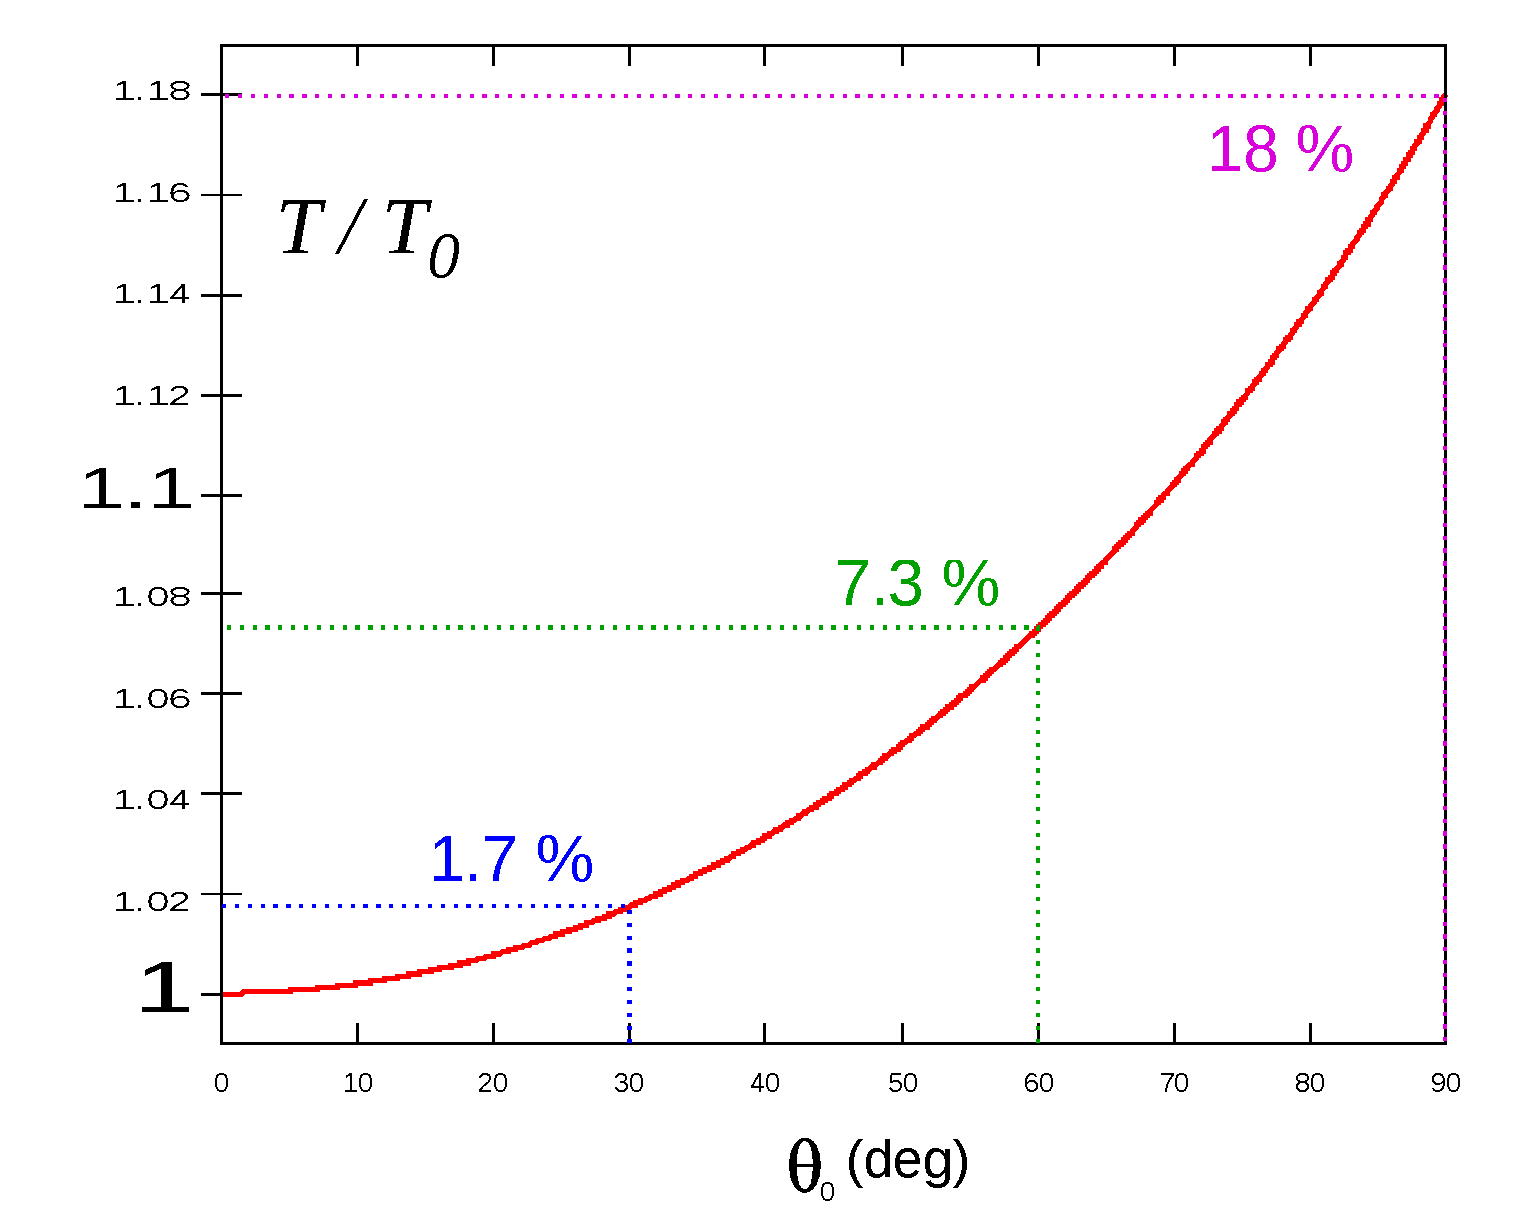
\includegraphics[width=0.6\textwidth]{images/ow-Pendulum_period.pdf}
\caption{单摆周期和振幅的关系,微幅摆动的周期可能近似看做与振幅无关}\label{fig: ow-单摆的周期和振幅的关系}
\end{figure}



这一事实从单摆的运动方程也能够看得出来,摆动过程中的总能量可以用角度$\theta$和它对时间的一阶导数共同给出:
\begin{equation}
E = \frac{1}{2}ml^2\left(\frac{d\theta}{dt}\right)^2-mgl\cos\theta
\end{equation}
在摆动过程中机械能守恒,所以总能量对时间的导数为零:
\begin{eqnarray}
\frac{dE}{dt} = ml^2\frac{d\theta}{dt}\frac{d^2\theta}{dt^2}+mgl\sin\theta\frac{d\theta}{dt}  = ml^2\frac{d\theta}{dt}\left(\frac{d^2\theta}{dt^2}+\frac{g}{l}\sin\theta\right)=0
\end{eqnarray}
从中可以看出摆动过程的运动方程为
\begin{equation}
\frac{d^2\theta}{dt^2}+\frac{g}{l}\sin\theta=0
\end{equation}
当摆动的角度时刻保持小角时,尤其是最大的摆动角,也就是振幅也可近似地看作是小角度时,摆动过程的方程就可以利用小角度近似而变成
\begin{equation}
\frac{d^2\theta}{dt^2}+\frac{g}{l}\theta=0
\end{equation}
它和弹簧振子振动过程的方程有着相同的形式,也可以与弹簧做类比推断出小角度摆动下周期与振幅无关的事实,并且可知单摆摆动的角频率和周期分别为
\begin{equation}
\omega = \sqrt{\frac{g}{l}},\qquad T = 2\pi\sqrt{\frac{l}{g}}
\end{equation}

\begin{example}
地球表面不同位置摆长一样的单摆微幅摆动的周期是否想同?如有不同请估计两极与赤道处周期差别。
\tagged{student}{\vspace*{4cm}}
\begin{taggedblock}{teacher}
\newline
解析:不一样,赤道g比较小,T大
\end{taggedblock}
\end{example}

\begin{example}
如图所示的有一个质量为$m$的物体被一根长度为$l$不可伸长质量忽略不计的绳挂于$O$点,与此同时它还与一端固定在它的最低点处原长为0劲度系数为$k$的弹簧连接,求它在作微幅摆(振动)的周期。
\tagged{student}{\vspace*{4cm}}
\begin{taggedblock}{teacher}
\newline
解析:以它偏离最低点的角度$\theta$标记物体的状态,这样整个系统的总能量由动能、重力势能和弹性势能共同给出:
\[
E = \frac{1}{2}ml^2\dot{\theta}^2+mgl(1-\cos\theta)+\frac{1}{2}kl^2\theta^2
\]
在小角度近似下$\cos\theta\simeq 1-\frac{1}{2}\theta^2$,这样总能量可以近似地写成
\[
E = \frac{1}{2}ml^2\dot{\theta}^2+\frac{1}{2}mgl\theta^2+\frac{1}{2}kl^2\theta^2
\]
由机械能守恒,$E$对时间的导数为零
\[
\frac{dE}{dt}=ml^2\dot{\theta}\ddot{\theta}+mgl\theta+kl^2\theta = ml^2\dot{\theta}(\ddot{\theta}+\frac{g}{l}\theta+\frac{k}{m}\theta)=0
\]
简化可得运动方程为
\[
\ddot{\theta}+(\frac{g}{l}+\frac{k}{m})\theta=\ddot{\theta}+\omega^2\theta=0
\]
这样可得振动的周期
\[
T = 2\pi\frac{1}{\sqrt{\frac{g}{l}+\frac{k}{m}}}
\]
\end{taggedblock}
\end{example}



\begin{example}
一个质量为$m$的质点作无阻力的一维运动,它所受外力由势函数$V(x)$所给出
\[f(x) = -\frac{dV(x)}{dx}\]
求证它在平衡位置附近作微幅振动的周期
\[T=2\pi\sqrt{\frac{m}{V''(x_0)}} \]
其中$V''(x_0)$为势函数在平衡位置上的二阶导数值。
\tagged{student}{\vspace*{3cm}}
\begin{taggedblock}{teacher}
\newline
解析:在平衡位置$x_0$处质点受到的保守力$f(x_0) = -\frac{dV}{dx}\bigg |_{x_0} = 0$,离开平衡位置则可能受到非零的外力。
无论如何力是位置的函数,当偏离平衡位置的程度很小时可以将力做近似展开,数学上就是用力作为位置的函数在平衡位置附近用它的切线来近似代表,这时可以认为物体受到回复力的作用。
切线的斜率
\[ \frac{df}{dx} = \frac{d}{dx}(-\frac{dV}{dx}) = -\frac{d^2V}{dx^2}\bigg |_{x_0}  \]
如果势能的二阶导数大于零,那么物体将受到线性的回复力,在回复力作用下将做简谐振动,根据简谐振动的一般规律,很容易证明上述结论。
\end{taggedblock}
\end{example}

\subsection{微幅振动}
其实从单摆的例子就能够看出,不仅是弹簧振子的位置,其实任何一个物理量在它的变化过程中满足和弹簧振子相同的方程,它在变化的过程中就满足和简谐振动相似的规律。
不失一般性将在一个物理问题当中感兴趣的物理量用$Q$表示,它的变化满足方程
\begin{equation}
\frac{d^2Q}{dt^2}+\omega^2Q=0
\end{equation}
那么运动方程的解可以表示成
\begin{equation}\label{eqn: ow-一般的振动}
Q(t) = A\cos\omega t+B\sin\omega t
\end{equation}
其中$A$和$B$是两个常数,它们由初始条件
\[
Q_0=Q(0),\qquad  v_0=\frac{dQ}{dt}(0)
\]
决定。
将初始条件代入方程一的一般解可以决定两个常数为
\[ A = Q_0,\qquad B = \frac{v_0}{\omega}. \]

对于一个能够作简谐振动的物理量$Q$,系统的势能在由$\frac{dV}{dQ}=0$决定平衡位置$Q_0$附近能表达或近似地表达为$Q$的二次函数:
\begin{equation}
V(Q) = V(Q_0+\varepsilon) = V(Q_0)+\frac{1}{2}\kappa\varepsilon^2,
\end{equation}
其中$\varepsilon$为振动的物理量与平衡位置的差别,系数$\kappa$可以表达为势函数$V(Q)$的二阶导数在$Q_0$处的值:
\begin{equation}
\kappa = \frac{d^2V}{dQ^2}\bigg|_{Q=Q_0}
\end{equation}
与此同时当$Q$随时间变化时整个系统的“动能”可以由它随时间的导数$\frac{dQ}{dt}$的二次函数
\begin{equation}
E_k = \frac{1}{2}\mu \left(\frac{dQ}{dt}\right)^2=\frac{1}{2}\mu \left(\frac{d\varepsilon}{dt}\right)^2
\end{equation}
给出,与弹簧振子相比较能够发现物理量$Q$的变化满足方程\ref{eqn: ow-一般的振动},其角频率和周期分别为
\begin{equation}
\omega = \sqrt{\frac{\kappa}{\mu}},\qquad T = 2\pi\sqrt{\frac{\mu}{\kappa}}.
\end{equation}

\begin{example}
如图所示,在两个相距$2L$的两个固定端点$A、B$点上连接两根劲度系数为$k$,原长$L_0<L$的弹簧,两根弹簧的另一端共同与一个质量为$m$的质点$P$连接,质点被限制在垂直于$AB$连线方向的轨道$MN$上运动,整个系统位于一个光滑平面上,求它在平衡位置附近做微幅振动的周期。
\begin{flushright}
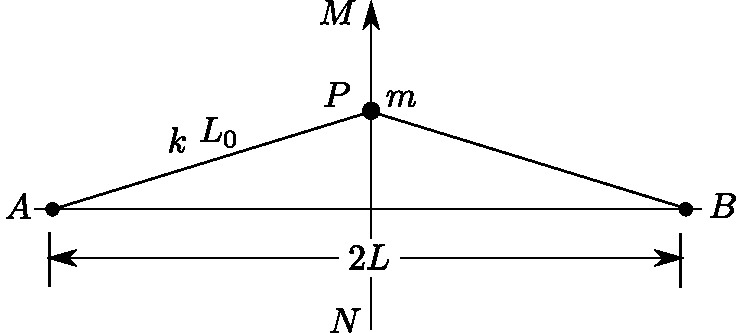
\includegraphics[width = 0.4\textwidth]{images/ow-two-springs-oscillation.pdf} 
\end{flushright}
\tagged{student}{\vspace*{3cm}}
\begin{taggedblock}{teacher}
\noindent
解析:就用上图所示的坐标系,当振子位于坐标$x$处时整个系统的势能只包含两根弹簧的弹性势能
\[V = 2\frac{1}{2}k(\sqrt{x^2+L^2}-L_0)^2,\]
其平衡位置由势能对x的导数为零的条件给出:
\[
\frac{dV}{dx} = 2k(\sqrt{x^2+L^2}-L_0)\frac{x}{\sqrt{x^2+L^2}}=0
\]
很明显$x=0$为它的解,在平衡位置处势能对$x$的二阶导数值
\[
\frac{d^2V}{dx^2}\bigg|_{x=0} = \frac{2k(L-L_0)}{L},
\]
这样微幅振动的周期就等于
\[
T = 2\pi\frac{mL}{2k(L-L_0)}
\]
\end{taggedblock}
\end{example}

\begin{example}
一个质量为$m$,原长为$L$的弹簧悬挂在$O$点,求它平衡时最低点与悬挂点的距离以及在平衡位置附近作微幅振动的周期。

\tagged{student}{\vspace*{3cm}}
\begin{taggedblock}{teacher}
\noindent
解析:建立一个原点在悬挂点、竖直向下的坐标轴,用弹簧另一端点的坐标来表示弹簧的位置。
弹簧的势函数在该坐标系当中可以写成
\[
V(x) = -mg\frac{x}{2}+\frac{1}{2}k(x-L)^2
\]
将它对$x$求导可得平衡位置:
\[
\frac{dV}{dx} = -\frac{1}{2}mg+k(x-L)=0,\qquad x_0 = \frac{mg}{2k}+L
\]

当弹簧在振动时,它的动能和势能均会随着端点的移动发生变化。
如果端点的坐标为$x$,速度为$\dot{x}$,它的动能可以通过积分
\[
E_k = \int_0^x \frac{1}{2}(\frac{m}{L}d\xi)(\frac{\xi}{x}\dot{x})^2 = \frac{1}{6}m\dot{x}^2
\]
这样总能量就是
\[
E = E_k+V = \frac{1}{6}m\dot{x}^2-mg\frac{x}{2}+\frac{1}{2}k(x-L)^2
\]
能量守恒可以给出运动方程
\[
0=\frac{dE}{dt} = \frac{1}{3}m\dot{x}\ddot{x}-\frac{1}{2}mg\dot{x}+k(x-L)\dot{x},\qquad \frac{1}{3}m\ddot{x}-\frac{1}{2}mg+k(x-L)=0
\]
将坐标表示为
\[
x = x_0+\varepsilon
\]
运动方程可以进一步变成
\[
\ddot{\varepsilon} +\frac{3k}{m} \varepsilon = 0
\]
很明显振动的周期可以写成
\[
T = 2\pi\sqrt{\frac{m}{3k}}
\]

\end{taggedblock}
\end{example}

%%%%%%%%%%%%%%%%%%%%%%%%%%%%%%%
\subsection{阻尼、受迫振动,共振}
前面讨论的各种例子当中可以看出简谐振动非常具有普遍性,很多的自然现象都是严格或近似的简谐振动。
但之前分析的振动过程是非常理想的情况:物体在无阻力和外力的情况下自由振动,真实的振动过程中不可避免地受到阻力和外力。
受阻力影响的振动称作\emph{阻尼振动},在阻力影响下能量不断地损失,相应地振幅必将不断地减小,一般来说振动现象最终将停止,当物体所受阻力仅正比于其速度时振幅有着相对简单的衰减规律。
受外力影响的振动称为\emph{受迫振动},这时振子的运动规律由其自身的动力学性质和外力共同决定,不同的外力引起振动性质的改变不尽相同。
当周期性外力作用于振子时振动的振幅不仅与外力的大小有关,外力的频率也将对受迫振动的振幅有影响,当外力的频率与振子的固有频率接近时会引起很大的振幅,这种现象称为\emph{共振}。


\begin{example}
如图所示,粗糙水平表面上有一弹簧振子,弹簧弹性系数为$k$,振子的质量为$m$,平面的摩擦系数为$\mu$,试定性地分析振动的行为。
设弹性系数$k=1\unit{N/m}$,$m=1\unit{kg}$,$\mu=0.01$,若开始时将弹簧向右侧拉开$1\unit{m}$,试求最终停止的位置,简单起见设$g=10\unit{m/s^2}$。
\tagged{student}{\vspace*{3cm}}
\begin{taggedblock}{teacher}
\newline
解析:平衡点位置变化的简谐运动。最后停在弹簧原长处。
\end{taggedblock}
\end{example}


\begin{example}
一个质量为$m$在劲度系数为$k$的弹性力$f=-kx$和正比于速度的阻力$f=-\alpha v$共同作用下作受迫振动。
受迫振动的运动方程可以写作
\[
\frac{d^2x}{dt^2}+\beta\frac{dx}{dt}+\omega_0^2x=0,
\]
试通过给定物理量决定上式中的$\beta$和$\omega_0$,进一步证明
\[
x(t) = e^{-\frac{\beta}{2}t}\left[ A\cos\left(\sqrt{\omega_0^2-\frac{\beta^2}{4}}t\right)+B \sin\left(\sqrt{\omega_0^2-\frac{\beta^2}{4}}t\right) \right]
\]
为方程的解,其中$A$、$B$为两个任意的常数。并画出x(t)的图像。
%受迫振动的图像如下,根据上面的解给出图中虚线的方程。

\tagged{student}{\vspace*{3cm}}
\begin{taggedblock}{teacher}
\noindent
解析:略
\end{taggedblock}
\end{example}


\begin{example}
质量为$m$在劲度系数为$k$的弹簧力$f=-kx$和周期的外力$f(t)=f_0\sin\omega t$作用下作受迫振动,试证明振动过程的运动方程可以写为
\[
\frac{d^2x}{dt^2}+\frac{k}{m}x=\frac{d^2x}{dt^2}+\omega_0^2x=\frac{f_0}{m}\sin\omega t,
\]
假设振动方程的解能够写为
\[
x(t) = A\sin\omega t+B\cos\omega t
\]
的话,将其代入运动方程决定$A$和$B$与有关参数的关系。
你会发现在一个特殊情况下上述方程无解,试解释这一现象并提出对方程的改进方案。
\tagged{student}{\vspace*{3cm}}
\begin{taggedblock}{teacher}
\newline
解析:将试探解代入运动方程可得
\[
-\omega^2 A \sin\omega t-\omega^2 B\cos\omega t+\omega_0^2A\sin\omega t +\omega_0^2 B\cos\omega t=\frac{f_0}{m}\sin\omega t
\]
因为正弦和余弦相互独立,所以要想上式成立,对应的系数必须均为零:
\[
-\omega^2 A+\omega_0^2 A = \frac{f_0}{m},\qquad -\omega^2 B+\omega_0^2 B=0 
\]
很明显它的解是
\[
A = \frac{f_0}{m}\frac{1}{\omega_0^2-\omega^2},\qquad B=0
\]
从中可以看到当策动力的频率和弹簧的固有频率相同时$A\rightarrow \infty$,无解!
这是因为忽略了一个重要的现象:振动的阻尼,当考虑了阻尼之后将会得到一个有意义的解。
\end{taggedblock}
\end{example}







\section{波}
一般来说振动的质点会和周围的物质有或大或小的相互作用,这样当质点发生振动时它会通过这些相互作用将它振动的能量传递给周围的物质。
这些被引起振动的物体又会导致更远处物体的振动,这样第一个物体的振动就以这样的方式不断地向外传递,就形成了波。
不夸张地说波是最广泛的自然现象,它几乎是整个宇宙能量和信息传递唯一的途径,所有的物质都具有或多或少的波动性。
自然界中的波主要包括两大类,\emph{机械波}是依靠构成介质的原子分子之间相互作用传递的波动现象,介质受力以后其内部结构会发生变形,而这种形变会以波的形式传递开来,典型的机械波包括固体内部的振动、声波等。
除了机械波以外还有著名的\emph{电磁波},它表现为光的传播,带电物质的运动产生光,光可以依据其自身的规律在真空当中传播,正是因为这个特点宇宙中不同天体之间的能量主要依靠电磁波来传递。
这里我们首先学习波的基本特点和简单的机械波,在学完电磁相互作用以后再来详细讨论电磁波。

\subsection{波的性质}

和质点振动不同的是在机械波传递过程中有大量的质点同时发生振动。
依据振动方式的不同波又分为横波和纵波:振动方向和波传播方向垂直的波称为\emph{横波},反之振动方向和传播方向平行的波则称为\emph{纵波}。
图\ref{fig: ow-横波和纵波}给出了用普通的弹簧演示的横波和纵波的例子,一端被上下振动的弦和电磁波是典型横波的例子,而声波则是具有代表性的纵波。

\begin{figure}[hbtp]
\centering
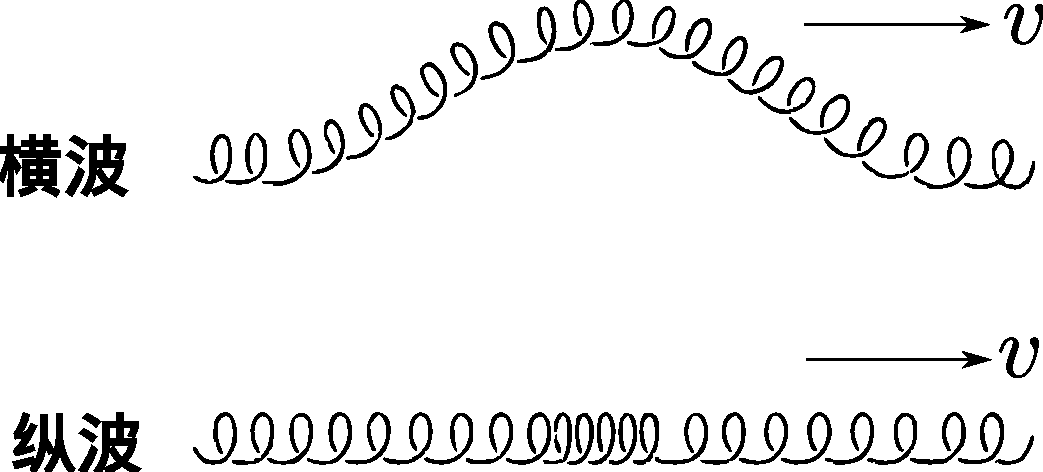
\includegraphics[width=0.6\textwidth]{images/ow-1.pdf}
\caption{横波和纵波}\label{fig: ow-横波和纵波}
\end{figure}

波是能量的传递,根据波动到达空间中各个点时间的不同也能够对波进行分类。
这其中最为简单的传递方式包括平面波和球面波。
当处于均匀介质中的单个质点发生振动时,它所引起的振动效果到达不同方向相同距离处的时间均相同,我们说它发出了\emph{球面波},在介质中传递的波一般来说具有叠加性,即来自不同波源的波在同一点引起的振动可以看成是单个波源产生振动效果的叠加,从这个意义上讲所有的波都是球面波的叠加。
数学上球面波有一定的复杂性,但如果考察的点与波源的距离很远时,单个波源发出的球面波可以用平面波来近似表示。
图\ref{fig: ow-球面波的平面波}给出了球面波和平面波的图形,其它的波形过于复杂,需要专门的数学工具才能够处理。

\begin{figure}[hbtp]
\centering
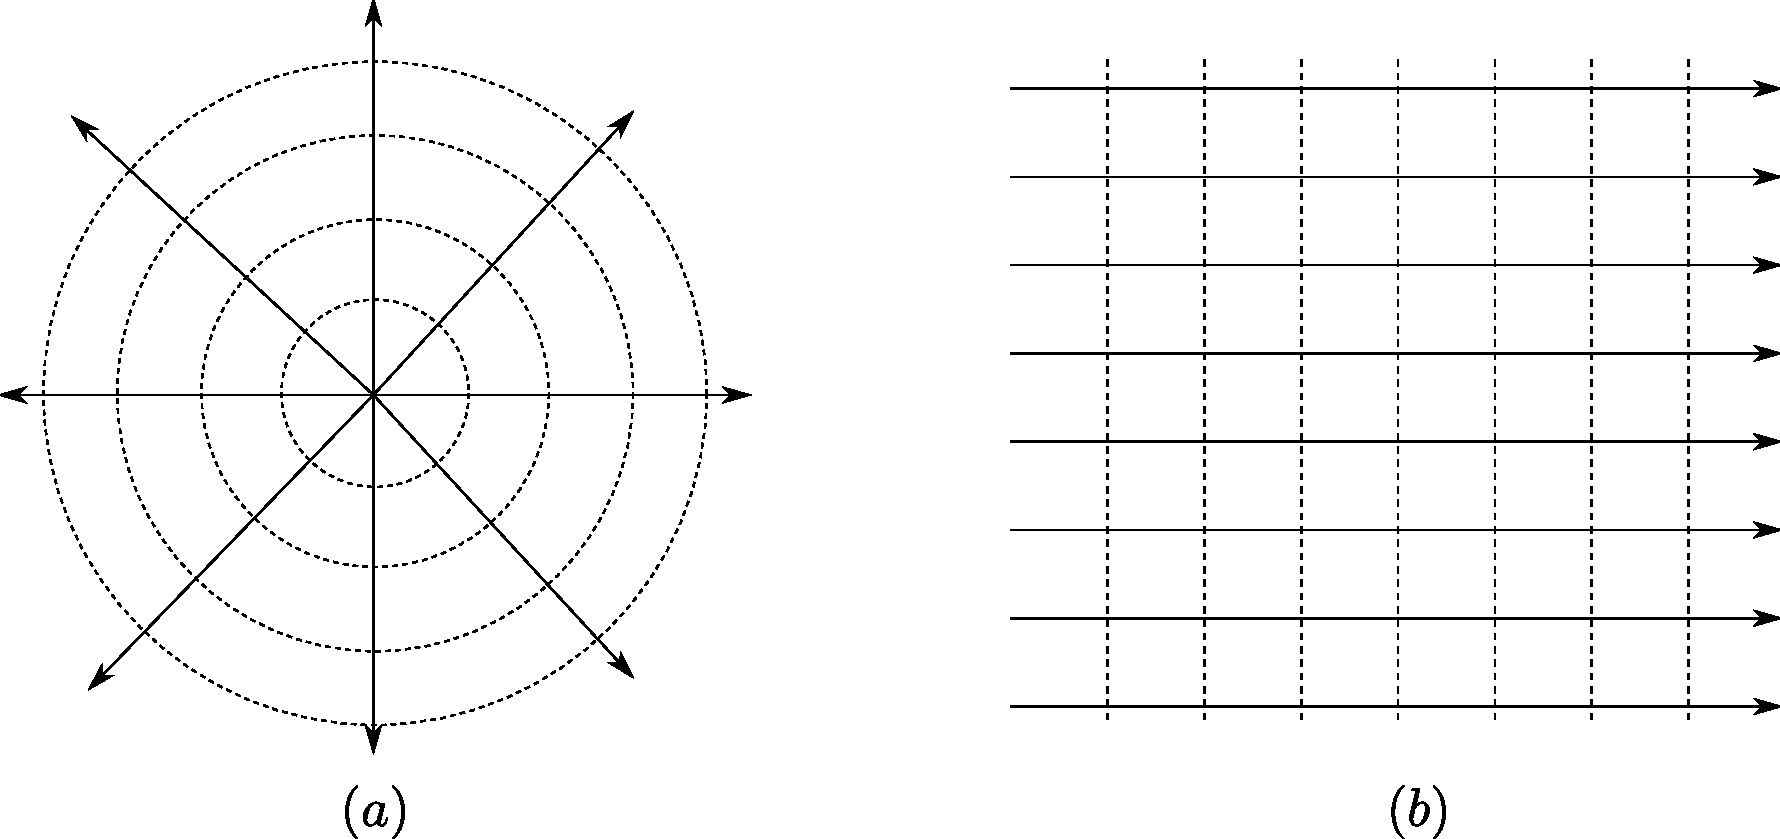
\includegraphics[width=0.6\textwidth]{images/ow-2.pdf} 
\caption{球面波和平面波,虚线代表相同时间以相同方式振动的部分,实线是波传播的方向}\label{fig: ow-球面波的平面波}
\end{figure}

所有的波动现象中属沿一条给定直线的无衰减、无扩散且具有单一频率的平面简谐横波最为简单,它为研究其它复杂波动现象提供了术语和样本。
如图所示的一个平面正弦横波沿$x$轴方向传播,振动方向则是图中的$y$轴,这样质点沿$y$方向的位移由它所处的位置$x$和时间$t$共同决定:
\begin{equation}\label{eqn: ow-最简单的横波}
y(x,t) = A\cos(\omega t-k x +\varphi),
\end{equation}
其中$A$称为波的\emph{振幅},$\omega$为波的角频率,$k$称为\emph{波数},$\varphi$为波的\emph{相位},它们一起决定了一个波的性质。

波的表达式\ref{eqn: ow-最简单的横波}是一个位置和时间的多元函数,为了清楚地看到波的特征,开始的时候固定其中的一个变量是一个好的主意。
首先来看$x$轴上一个给定点$x_0$的变化行为,在该点处质点位移是时间的函数
\begin{equation}
y(x_0,t) = A\cos(kx_0-\omega t +\varphi)
\end{equation}
从中可以波传递线路上的每个质点都在作简谐振动,简谐振动的振幅与波的振幅$A$一致,角频率也是波的角频率$\omega$,但是各个点振动的相位则不但与波的相位$\varphi$有关,也与它的位置$x_0$有关。
给定点上质点振动的频率也称为波的频率,频率一般用$f$来表示,它和角频率之间有关系
\begin{equation}
f = \frac{\omega}{2\pi}=\frac{1}{T}
\end{equation}
其中$T$是一点简谐振动的周期,它也是波的周期。
与$x_0=0$的质点振动的相位相比较可以看出,$x_0>0$处质点振动的相位会落后$kx_0$。

对于给定的时间$t_0$,所有点的位移为
\begin{equation}
y(x,t_0) = A\cos(kx-\omega t_0+\varphi)
\end{equation}
它们共同构成$y-x$平面内的余弦函数的图像。
位移刚好达到正弦函数最大值的点称为\emph{波峰},反之到达最小值的那些点称为\emph{波谷},相邻两个波峰或波谷之间的距离称为\emph{波长},习惯上用$\lambda$来表示,从上式可以看出波长和波数之间满足关系
\begin{equation}
\lambda = \frac{2\pi}{k}.
\end{equation}
波长是波最重要的物理量之一,很多现象都与波长密切相关。

波的振幅也和波在传递过程中携带的能量密切相关,和简谐振类似波的能量正比于振幅的平方。
在大多数情况下这个比例系数并不是特别地重要,但能量和振幅的关系却对波的外部性质起着至关重要的决定性。

波的表达式\ref{eqn: ow-最简单的横波}自变量可以重新组合成
\begin{equation}
y(x,t) = A\cos\left[k(x-\frac{\omega}{k}x)+\varphi)\right] = A\cos\left[k(x-\lambda f \cdot t)+\varphi)\right]
\end{equation}
上式可以解释为对于那些$x-\lambda f t$取相同值的点上振动质点的位移均相同。
形象地看随着时间的推移余弦函数的图像向右移动,从时刻$t$开始算起当再经过$\Delta t$时间以后,那些与$t$时刻位移完全相同的点的横坐标偏移量可由
\[
x-\lambda f t = x+\Delta x-\lambda f (t+\Delta t)
\]
给出,简单的代数运算可以得到
\[
\Delta x = \lambda f \cdot\Delta t,
\]
波长和频率的乘积可以看成波的图像向右运动的速度,称为\emph{波速}$v$,它们三个物理量之间满足关系式:
\begin{equation}\label{eqn: ow-v=lambad f}
v = \lambda f
\end{equation}
波速是描写波的性质的另外一个重要的物理量,声波的速度称为声速,光波的速度称为光速,将来我们会看到在物理学中光速扮演着至关重要的角色。

\begin{example}
已知一列平面波可以用方程
\[y(x,t) = (1\unit{cm})\cdot\cos\left[(5\unit{s^{-1}})t-(10\unit{cm^{-1}}) x+\frac{\pi}{2}\right ]\]
来描写,请给出这列波的振幅、频率、周期、波长、波速、相位等相关的物理量。
\tagged{student}{\vspace*{4cm}}
\begin{taggedblock}{teacher}
\newline
解析:波的振幅$A = 1cm$可以直接求出。
根据定义,频率$f = \frac{\omega}{2\pi} = \frac{5}{2\pi}\unit{Hz}$,周期$T = \frac{1}{f} = \frac{2\pi}{5}\unit{s}$,波长$\lambda = \frac{2\pi}{k} = \frac{2\pi}{10}\unit{cm}$,波速$v = \lambda f = 0.5\unit{cm/s}$,最后相位可以直接从波的运动方程读出$\varphi = \frac{\pi}{2}$。
\end{taggedblock}
\end{example}


\begin{example}
已知一列沿着$x$轴正方向传递的横波其振幅为 $1\unit{cm}$,频率为$8\unit{Hz}$,波长为$30\unit{cm}$,在$t=0$的时刻位于$x=15\unit{cm}$处的质点刚好位于波峰位置,求此波的运动方程。
\tagged{student}{\vspace*{4cm}}
\begin{taggedblock}{teacher}
\newline
解析:从给出的信息可以通过计算得到波的角频率、波数和相位,最终确定波的运动方程。
振幅$A = 1\unit{cm}$直接可以得到,角频率$\omega = 2\pi f = 16\pi\unit{s^{-1}}$,波数$k = \frac{2\pi}{\lambda} = \frac{\pi}{15}\unit{cm^{-1}}$。
相位最难确定,$t=0$时$x=15\unit{cm}$处的质点运动方程应该是
\[y(t,x=15) =  A\cos(16\pi t -\pi +\varphi) \]
要想刚好处于平衡位置,需要$\varphi - \pi = \pi/2 \textbf{or} 3\pi/2$,这时质点的运动速度
\[ \frac{dy}{dt} = -A \sin(-\pi+\varphi)>0\]
这样唯一的可能就是$\varphi = \pi/2$,将上面的结果全部合起来得到波的运动方程
\[ y(x,t) = 1\cos(16\pi t - \frac{\pi}{15}x +\frac{\pi}{2})\]
其中时间的单位取秒,振幅和位置的单位取厘米方可。
\end{taggedblock}
\end{example}

\begin{example}
一列简谐波在均匀介质中沿$x$轴正方向传播,两质点$P_1$和$P_2$的平衡位置在$x$轴上,它们相距$60\unit{cm}$,当$P_1$质点在平衡位置处向上运动时,$P_2$质点处在波谷位置。
若波的传播速度为$24\unit{m/s}$,则该波的频率可能为$\underline{\qquad}$。

$A.\quad 50\unit{Hz}\qquad B.\quad 60\unit{Hz}\qquad C.\quad 400\unit{Hz}\qquad D.\quad 410\unit{Hz}$
\tagged{student}{\vspace*{4cm}}
\begin{taggedblock}{teacher}
\newline
解析:AD。根据已知条件可知两给定点之间的距离应当是波长的$n+\frac{1}{4}$倍,其中$n$为非负整数:
\[   (n+ \frac{1}{4} )\lambda = 0.6 \]
根据波速又可知波长和频率的关系为
\[  24 = \frac{0.6}{n+ \frac{1}{4} }f,\qquad f = 10(4n+1) \]
可以看出,频率值减去10需要可以被4整除方可,可得最终结果。
\end{taggedblock}
\end{example}

\begin{example}
已知一个沿$x$轴正方向以速度$v=2\unit{m/s}$传递的波在$t=0$时刻的波形如图所示,请定性画出$x=2$的质点位移随时间的关系。
\begin{center}
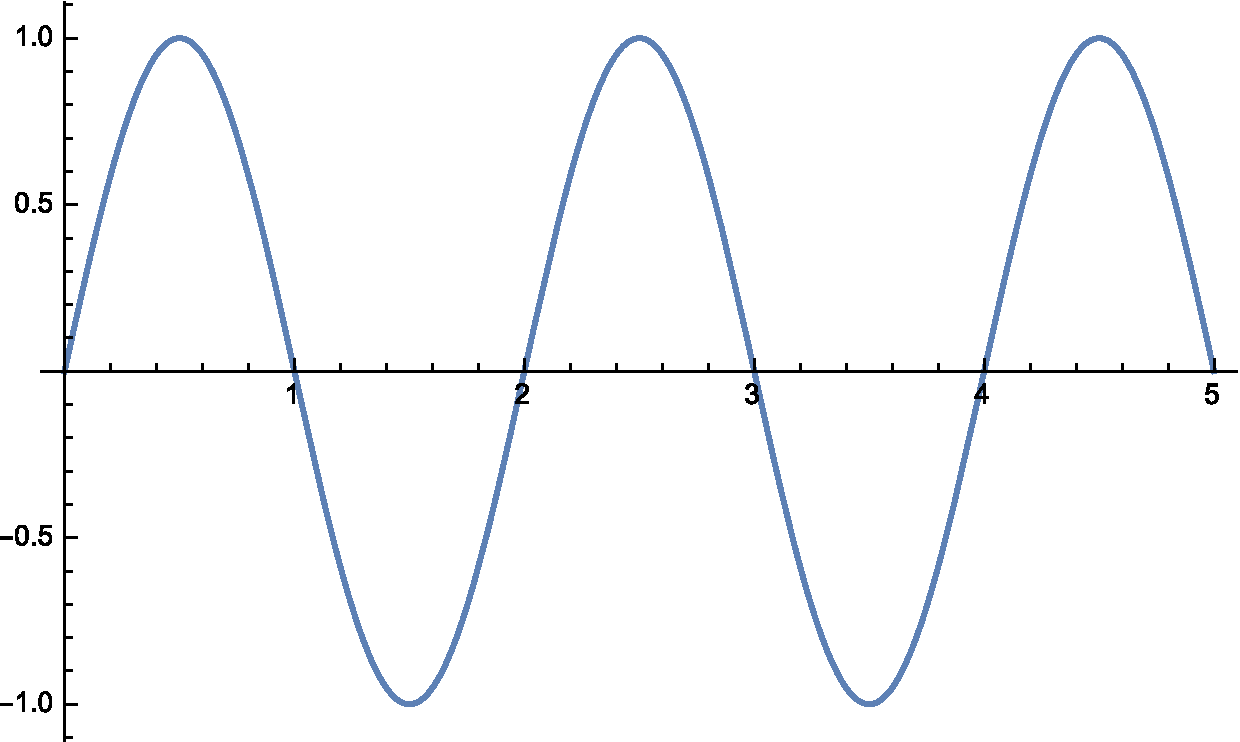
\includegraphics[width = 0.4\textwidth]{images/ow-problem-1.pdf}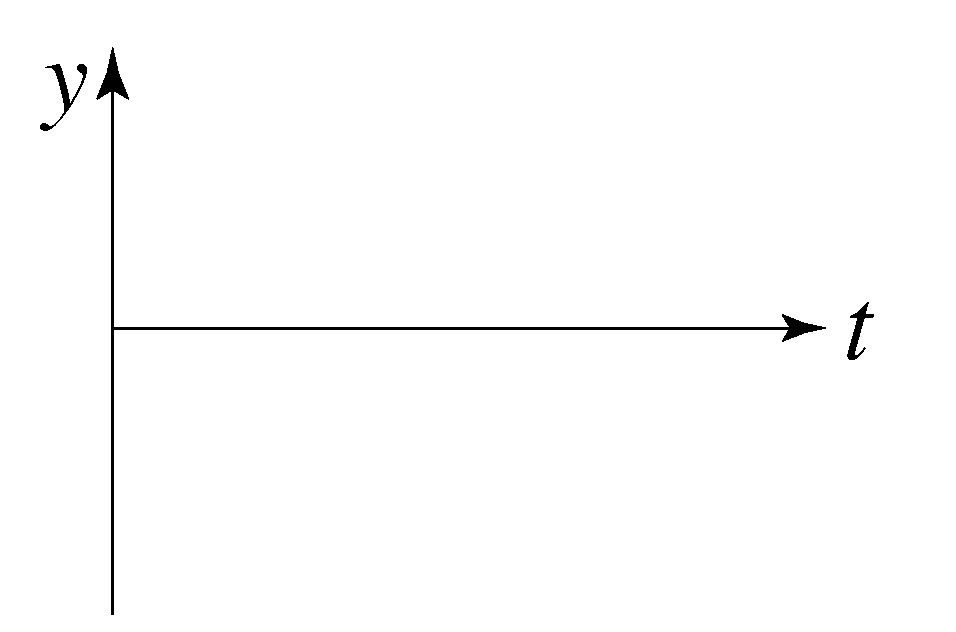
\includegraphics[width = 0.4\textwidth]{images/ow-problem-1-1.pdf}
\end{center}
\tagged{student}{\vspace*{1cm}}
\begin{taggedblock}{teacher}
\noindent
解析:简谐波传播路径上任何一点都随时间作简谐振动,$t=0$时$x=2$处的质点位于原点处,从波传播方向可以看出此后它将向着$y$轴负方向运动。
从$t=0$时刻的波形可以看出波长为 2,通过波速的信息可以确定每个质点振动的周期为1。
以上的信息足够画出$x=2$质点的振动状态。
\end{taggedblock}
\end{example}


\begin{example}
前面我们已知$y = A\cos(\omega t-kx)$可以用来描写一列沿着$x$轴正方向传递的波,那么沿着$x$轴负方向传递的相同振幅、相同波长和频率的波又该如何描写呢?
\tagged{student}{\vspace*{4cm}}
\begin{taggedblock}{teacher}
\newline
解析:在一维的时候不容易看出,实际上$k$是空间的一个矢量,对于平面波来说它的长度是$2\pi/ \lambda$,方向指向波的传递方向,对于最一般的波它在平面直角坐标系的三个轴上都会有投影。
这样沿着$x$轴负方向传递的波就可以直接通过波矢的这个意义写成:
\[y = A \cos(\omega t + kx.)\]
\end{taggedblock}
\end{example}

\subsection{波的干涉和衍射}
前面曾经提到波是能量的传递,这样波速自然就是能量传递的速度,而传递能量的大小可以用振幅来确定。
考虑在波的传播路线上$x_0$处有一个质量为$m$的质点随波运动,也就是说它的位移和波动的大小完全一致,这样任一时刻它的动能就是
\begin{equation}
E_k = \frac{1}{2}m\left(\frac{dx}{dt}\right)^2
\end{equation}
将波的方程\ref{eqn: ow-最简单的横波}代入上式可得
\begin{equation}
E_k(t)= \frac{1}{2}m\omega^2A^2\sin^2(\omega t-kx_0+\varphi)
\end{equation}
它的动能随时间而变化,这里我们感兴趣的是它在振动过程中动能的平均值
\begin{equation}
\overline{E_k} = \frac{1}{T}\int_0^T E_k(t) = \frac{1}{4}m\omega^2A^2
\end{equation}
不考虑其它更复杂的因素,从中可以看出波的能量正比于它在该点振幅的平方。
准确地讲前面的推理是很粗糙的,但是结果却是正确的。
沿波传递的方程有能量的流动,而单位时间里通过的能量正比于波振幅的平方!

如果一个质点受到来自于两个波源波的影响,那么该点对平衡位置的偏离则等于两个波源在同一时刻在该点位移之和,这称为波的叠加原理,事实证明大多数波在振幅很小的情况下都具有叠加原理。
简单起见设两个波源发出的波是相同方向、相同频率的横波,即使如此在最一般的情况下两个波源发出波的振幅和相位也可能不同,称它们相位的差别为\emph{相位差}。
每个波源单独存在时的波动方程为
\begin{equation}
y_i (x,t)= A_i\cos(\omega t-kx+\varphi_i)
\end{equation}
下标$i=1,2$代表两列波,从中可以看到在我们假设的情况下两列波的差别仅体现在振幅和相位上。
当叠加原理成立时空间当中各点的位移为两列波产生位移之和:
\begin{equation}
y(x,t) =  A_1\cos(\omega t-kx+\varphi_1)+ A_2\cos(\omega t-kx+\varphi_2)
\end{equation}
利用三角函数的性质上式又可以表达为
\[
y(x,t) = A \cdot \cos(\omega t-kx+\beta)
\]
其中
\begin{equation}
A = \sqrt{A_1^2+A_2^2+2A_1A_2\cos(\varphi_1-\varphi_2)},\qquad \tan\beta = \frac{A_1\sin\varphi_1+A_2\sin\varphi_2}{A_1\cos\varphi_1+A_2\cos\varphi_2}
\end{equation}
从中可以看到两列波叠加以后形成一个合成的波,它的波长和频率和原来的波完全相同,而振幅和相位则会发生变化。
特别地,当两列波振幅相等时$A_1=A_2=A_0$时上式可以简化为
\[
A = A_0\sqrt{2+2\cos(\varphi_1-\varphi_2)} = 2A_0\cos\frac{\varphi_2-\varphi_1}{2} = 2A_0\cos\frac{\Delta \varphi}{2} ,
\]
其中$\Delta \varphi$称为两列波的\emph{相位差}。
 因为对于波来说它振幅的平方对应于该点处的能量,所以此时波在各点的能量最小为零,而最大为单个波存在时的4倍。
可以看到当两列波的相位差为$2\pi$的整数倍时,$A=2A_0$,此时能量取最大值,为单个波存在时的四倍;反之当相位差为$(2n+1)\pi$时$A=0$,所有的质点不发生位移,自然能量为零。
这就是波的\emph{干涉}现象,图\ref{fig: ow-波的干涉}给出了波的干涉的一个例子。

\begin{figure}[ht]
\centering
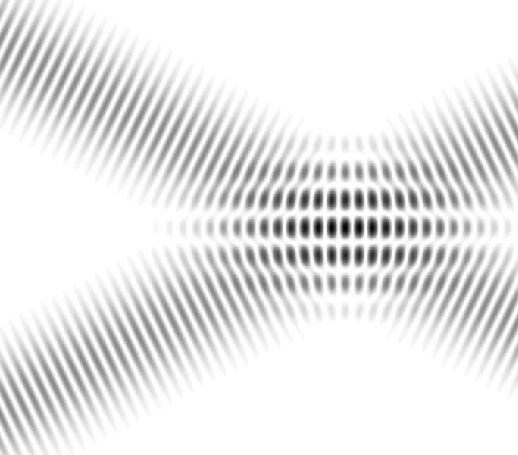
\includegraphics[width=0.5\textwidth]{images/Interferences_plane_waves.pdf}
\caption{干涉现象的一个例子}\label{fig: ow-波的干涉}
\end{figure}


\begin{example}
定性解释球面波的各点的振幅与它和波源的距离成反比。
\tagged{student}{\vspace*{4cm}}
\begin{taggedblock}{teacher}
\newline
解析:因为波的能量正比于振幅的平方,而球面波单位面积上的能量随着波远离波源而减小。
单位面积,单位时间里通过的能量与到波源距离的平方成反比,这样很容易看出球面波的振幅距离成反比。
\end{taggedblock}
\end{example}

\begin{example}
求两列由
\[y_1 = A\cos(\omega t-kx),\qquad A\cos(\omega t + kx +\varphi)\]
所给出的相向运动的平面波叠加之后的波的运动方程,并分析其运动学性质。
已知三角函数满足以下的恒等式:
\[\cos\alpha+\cos\beta = 2\cos\frac{\alpha+ \beta}{2}\cos\frac{\alpha- \beta}{2}\]
\tagged{student}{\vspace*{4cm}}
\begin{taggedblock}{teacher}
\noindent
解析:直接把两列波代入三角函数的和差化积公式中可得两列波叠加后的运动
\begin{eqnarray*}
y = y_1+y_2 = 2A\cos(\omega t +\frac{\varphi}{2})\cos(kx +\frac{\varphi}{2})
\end{eqnarray*}
从中可以看出这种情况下时间和空间变量被完全分离开来,每个质点都作简谐振动,但是振幅与位置有关。
\end{taggedblock}
\end{example}

\begin{example}
试定性地分析两列振幅不同但频率和波长均相同,沿相反方向传递的平面波叠加之后波的运动方向,并通过定量计算验证你的结论。
\tagged{student}{\vspace*{4cm}}
\begin{taggedblock}{teacher}
\newline
解析:因为波所携带的能量正比于振幅的平方,两列波迎面相遇时,如果振幅相同,那么就会形成上一问所求的驻波,但如果振幅不同,则沿着两个方向传递能量有所不同。
这样叠加之后的波形依然会向着原先振幅大的那列波的方向移动,但移动的速度将会小一些。


\end{taggedblock}
\end{example}

\begin{example}
有两列沿着相同方向传递的平面波,它们的振幅和波速均相同,但频率有微小的差别
\[y_1 = A\cos(\omega_1 t-kx),\qquad A\cos(\omega_2 t + kx +\varphi),\qquad \Delta\omega = \omega_1-\omega_2\ll\omega_{1,2}\]
请定性地分析叠加之后的波形,并通过定量计算验证你的结果。
\tagged{student}{\vspace*{4cm}}
\begin{taggedblock}{teacher}
\newline
解析:振幅会随时间缓慢变化的驻波\[ A\cos(\omega_1 t-kx)+A\cos(\omega_2 t + kx +\varphi)=2A\cos(\frac{\omega_1+\omega_2}{2}t+\frac{\varphi}{2})\cos(\frac{\omega_1-\omega_2}{2}t-kx-\frac{\varphi}{2})\]

\end{taggedblock}
\end{example}



\subsection{多普勒效应}
当波源或观测者相对于介质运动时,发出或接收到的波的频率或波长会随着它们的运动状态的不同有所不同,所有这类现象统称为\emph{多普勒效应}。
对于机械波来说有两种典型的多普勒效应
\begin{enumerate}
\item 波源静止观测者运动的情况:如图\ref{fig: ow-波源静止观测者运动时的多普勒效应}所示,设波源$S$相对于介质处于静止状态,观测者以速度$u$向着波源运动,这种情况下它接连两次遇到波峰的时间要短于波的周期,同理它看到波的频率$f'$则高于波相对于介质的频率$f$:
\begin{equation}
f' =\left(1+\frac{u}{v}\right)
\end{equation}
同理当观测者背对波源运动时,它所观测到的波的频率$f'$则小于$f$:
\begin{equation}
f'=f\left(1-\frac{u}{v}\right)
\end{equation}
这时当运动速度$u$超过波速$v$时,通过上式得到的频率为负值,物理上这意味着背对波源运动的物体将追上之前发出的波。
\begin{figure}[hbtp]
\centering
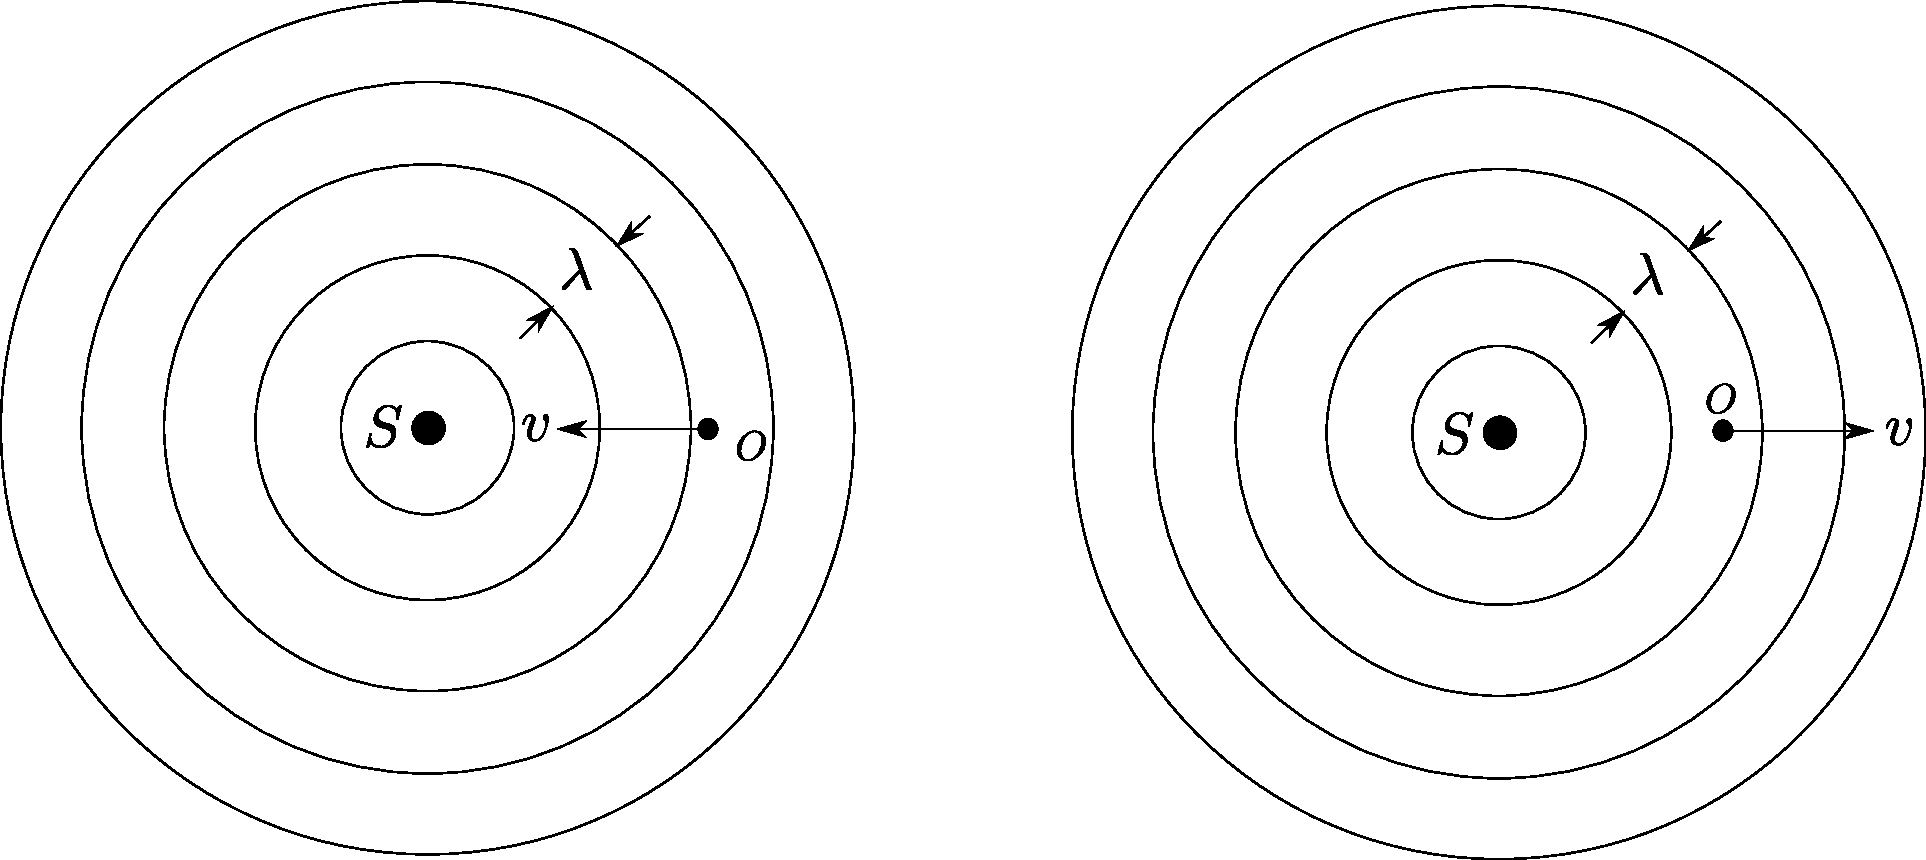
\includegraphics[width=0.6\textwidth]{images/ow-doppler-effect-observer.pdf}
\caption{波源静止观测者运动时的多普勒效应}\label{fig: ow-波源静止观测者运动时的多普勒效应}
\end{figure}

\item 波源运动而观测者静止的情况:波相对于介质传播速度不会发生变化,当波源运动时各个时刻的波前会由于波源的运动发生变形。
图\ref{fig: ow-波源相对介质运动时的多普勒效应}给出了波源速度小于、等于和大于介质中波速时波前的图形,简单的数学分析可以得出当波源向着静止观测者运动时观测者看到的频率
\begin{equation}
f' = \frac{1}{1-\frac{u}{v}}f
\end{equation}
同理当波源远离观测者时观测者测量到的频率则是
\begin{equation}
f'=\frac{1}{1+\frac{u}{v}}f.
\end{equation}
从图\ref{fig: ow-波源相对介质运动时的多普勒效应}(b)、(c)中可以看到当波源向着观测者运动速度超过波速时在波源运动到观测者所处位置之前观测者是看不到任何波动现象的,表现在数学公式上就是上面第二个式子在$u>v$时得到的结果没有物理意义。


\begin{figure}[hbtp]
\centering
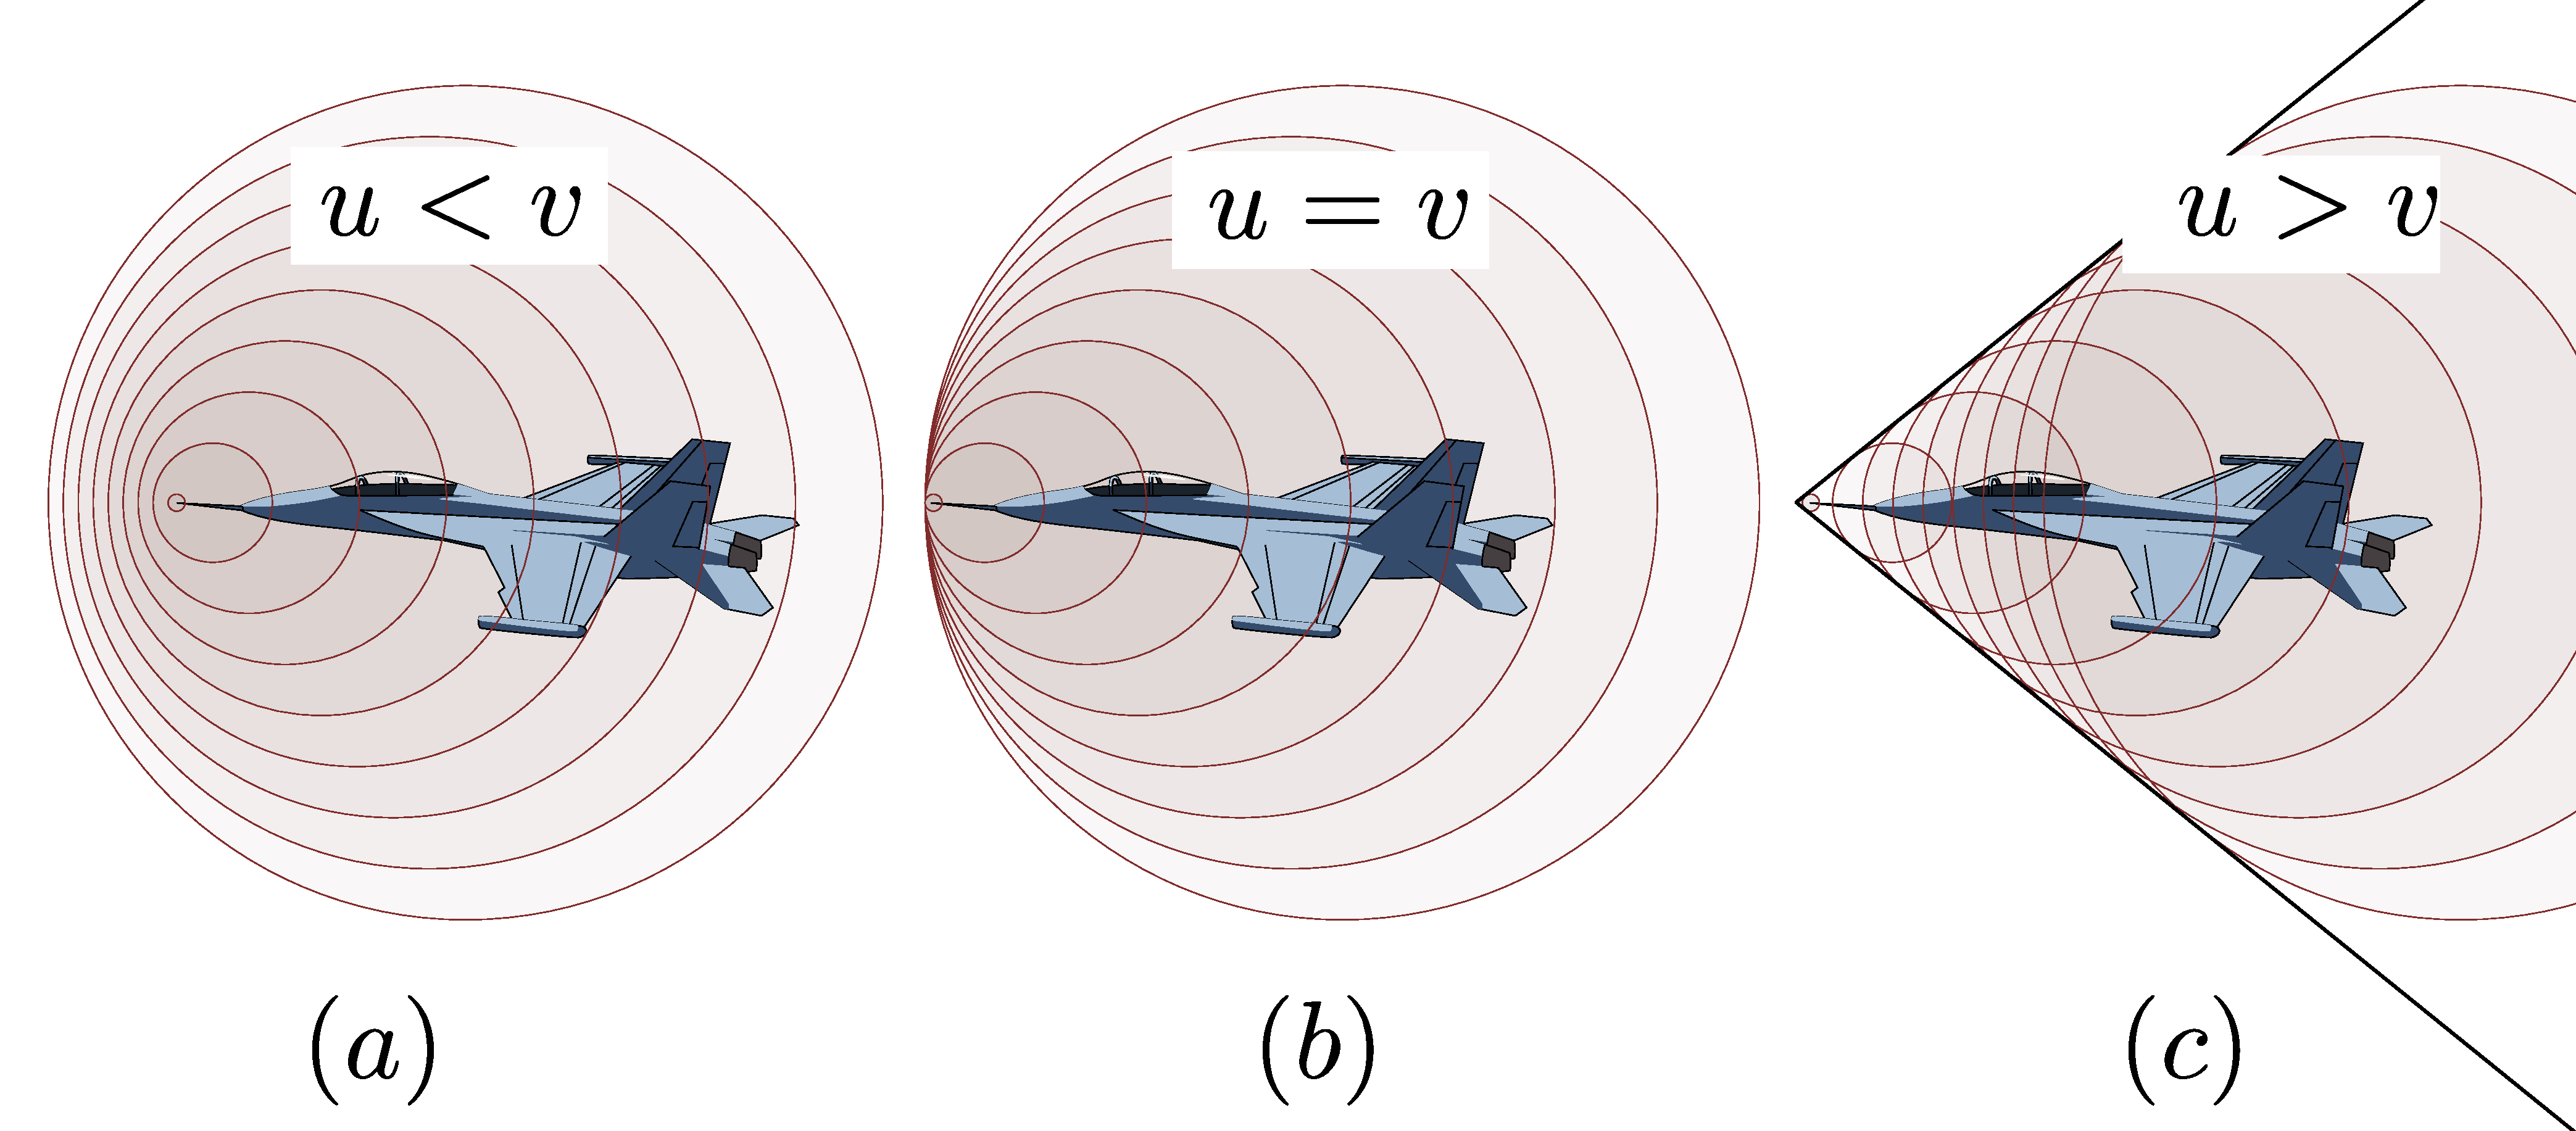
\includegraphics[width=0.7\textwidth]{images/ow-3.pdf}
\caption{波源相对介质运动时的多普勒效应}\label{fig: ow-波源相对介质运动时的多普勒效应}
\end{figure}

\end{enumerate}

\begin{example}
已知空气中的声速为$u$,有两架亚音速飞机一前一后在一条直线上飞行,它们的速度分别为$v_1$和$v_2$并且$v_{1,2}<u$。
它们各自发出频率为$f$的波,求每一架飞机接收到另一架飞机发出声波的频率。
如果它们是对向飞行,情况又如何?相互远离的情况分别接收到的频率又会发生什么样的变化呢?
\tagged{student}{\vspace*{4cm}}
\begin{taggedblock}{teacher}
\newline
解析:简单地多次使用上面的多普勒效应的结论即可得到所有的结果。
\end{taggedblock}
\end{example}

\begin{example}
当一架飞机以超音速飞行时,它所发出声波的波阵面将不再是一个球面,而是如图\ref{fig: ow-波源相对介质运动时的多普勒效应}所示的一个圆椎体的侧面,已知声速为$u$,超音速飞机飞行相对空气的速度为$v$,求图中椎体的顶角$\alpha$
\tagged{student}{\vspace*{4cm}}
\begin{taggedblock}{teacher}
\newline
解析:只需要画出波阵面和超音速飞机在给定时间里的运动,就可以马上看出椎角
\[  \sin\alpha  = \frac{u}{v}\]
\end{taggedblock}
\end{example}

电磁波的多普勒效应与机械波有不同,这和电磁波,也就是光的传播本质上不需要介质有很大的关系。
关于这一点我们将在掌握了电磁波更多的物理规律以后再来详细讨论。




\subsection{波的动力学}
上面给出了波的描述方式,叠加原理以及当波源或波的接收者相对于介质有运动时波性质的改变。
接下来简单地分析一个形成波的动力学机制,因为机械波的传播本质上是由构成介质物质之间的相互作用所导致,所以波的性质很大程度上是由介质自身的性质所决定。
通过下面几个例子我们将看到,介质的动力学性质将决定在其内部传递的机械波的波速,而波
的频率则是由波源的频率所决定。
因为波长、频率和波速三个量之间由方程\ref{eqn: ow-v=lambad f}相联系,所以波长并不是一个独立的物理量,当频率和波速被给出了以后,波长就被唯一决定。
另外波的振幅是由波源在单位时间里所提供的能量,也就是波源的功率决定,这一点通过振幅与能量的关系很容易理解;最后波的相位则完全由波源的初始状态给出。

\begin{example}
考虑一个简单化的介质模型,它由许多用几乎不可伸长的绳子连接起的质点构成。
每个质点的质量均为$m$,绳长为$l$,在绳子当中有张力$T$,试证明当这样一个简单介质中存在有一列振幅很小但波长$\lambda \gg l$的横波时,波速$v=\sqrt{Tl/m} = \sqrt{T/\rho}$,其中$\rho=m/l$为介质的线密度,也就是说波速完全由介质的参数给出,与其中传递的波的频率或波长无关。

(提示:余弦函数在一点处有近似的展开式$\cos(x+\Delta x)\simeq \cos(x)-\sin(x)\Delta x-\frac{1}{2}\cos(x)(\Delta x )^2$,其中$x$代表任何一点,$\Delta x$为$x$的微小变化量且$\Delta x\ll x$。)
\tagged{student}{\vspace*{8cm}}
\begin{taggedblock}{teacher}
\begin{center}
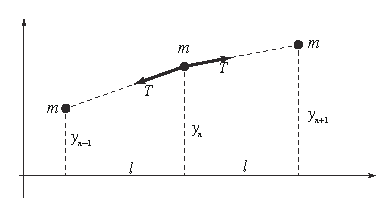
\includegraphics[width = 0.5\textwidth]{images/ow-solution-4-transverse-waves}
\end{center}
\noindent
解析:当各个质点的位置发生变化时,它们的相对位置关系如图所示。
我们给每个质点编上号,着重考察相邻的三个质点 $n-1$,$n$,$n+1$三个质点。
它们之间有张力作用,因为假设,它们在$y$方向的位移与$l$比起来可以忽略不计,所以张力的水平方向合力可以近似看做为零。
但是当它们三个点不在一条直线上时,则会有非零的$y$方向的合力。
根据受力的大小和方向,可以得出第$n$个质点在$y$方向的合力
\[F_n = \frac{T}{l}(y_{n-1}+y_{n+1}-2y_n)\]
它导致了第$n$个质点在$y$方向上的加速度。

假设介质中有横波,设波的运动方程为$y = A\cos(\omega t-kx)$,这时我们关注的三个质点的运动可以近似地看成
\begin{eqnarray*}
y_{n-1} &=&A\cos(\omega t - kx_n+kl)\simeq A\cos(\omega t - kx_n)-A\sin(\omega t - kx_n)(kl)-\frac{1}{2}\cos(\omega t - kx_n)(kl)^2\\
y_{n+1} &=&A\cos(\omega t - kx_n-kl)\simeq A\cos(\omega t - kx_n)-A\sin(\omega t - kx_n)(-kl)-\frac{1}{2}\cos(\omega t - kx_n)(-kl)^2\\
y_n&=&A\cos(\omega t - kx_n)
\end{eqnarray*}
将它们代入第$n$个质点的合外力表达式很容易得到此时合外力为
\[
F_n =- \frac{T}{l}k^2l^2y_n
\]
很容易发现它正比于第$n$个质点的位移,必然会导致它作简谐振动。
因为我们已经假设介质中有波的传递,所以此时简谐振动的角频率就是波的频率$\omega$,根据它的运动方程可以得到以下等式:
\[
- \frac{T}{l}k^2l^2y_n = -m \ddot{y_n} = -m\omega^2 y_n
\]
由波长、频率和波速度的关系可知$\omega = kv$,所以上式可以进一步化简为
\[
v^2 = \frac{Tl}{m} = \frac{T}{m/l} = \frac{T}{\rho}
\]
\end{taggedblock}
\end{example}


\begin{example}
考虑另一种简化的介质模型,它是由多个质量为$m$的质点由原长为$l$,弹性系数为$k$的细弹簧连接,其自然状态下每个弹簧均处于原长。
求介质中传递纵波的波速。
\tagged{student}{\vspace*{4cm}}
\begin{taggedblock}{teacher}
\newline
解析:这里的纵波传递和前面一问的横波其实极为相似,只需要注意到第n个质点在纵向振动的位移$y_n$应当表达为它偏离平衡位置的距离,还有就是它受到两边质点的弹性力可以表达为
\[F = k(y_{n-1}+y_{n+1}-2y_n)\]
其它的和前面的推理都是一样的,所以只需要将前面的$T/l$全部换成$k$即可。
所以介质中纵波的波速
\[
v^2 = \frac{kl^2}{m}
\]
这两个量均为微观量,实际上上式上下同时除以$l$,分子就变成了单位长度的弹性系数,分母则变成了质量线密度,因为它们是宏观量所以更具有实际意义。
\end{taggedblock}
\end{example}

前面讨论的都是一些理想情况,真实的波在传播过程中所面临的情况要复杂地多。
在此提出一些在将来的学习过程中可能出现的波动过程中需要考虑的因素,在遇到的时候再详细讨论
\begin{enumerate}
\item 振幅随位置的变化:因为波的振幅是衡量波所携带能量大小的物理量,所以除了平面波以外其它的波动过程中振幅必然会随着位置的不同而不同。
例如对于球面波来说,它的能量全部来自于波源,如果波在各向同性的介质中传递时,其能量必然会随着与波源距离的增加而减小,简单的定量分析可以得出球面波各点的振幅反比于到波源的距离。

\item 波的衍射:当波在传递过程中遇到障碍物时,尤其在遇到图所示的小孔会发生传播方向的变化,称为波的衍射。
波的衍射使其传播方向偏折,在天文观测中会影响光学仪器的分辨率。


\item 波的合成:真实的波源很难发出只有一种频率的波,而是多种频率波的叠加。
例如在演唱时同样的一个音符,男低音和女高音听起来很不相同;生活中很容易通过声音辨别出说话的人,这里面的原因就是它们发出声音中各种频率的波所占的比例各不相同,声学中将声音的这个特征称作\emph{音品}。
通过接收到的波信号分析其中各种频率所占的比例是一门专门的学科,今后会碰到一些这里面的例子。

\item 波的色散:因为真实的波一般来说包含各种频率的分量,而在介质中传播时不同频率或波长的波速一般来说不尽相同,由于不同波长的波速不同,所以在波的传播过程中各种波长的波会逐渐散开,这个现象称为波的\emph{色散}。
牛顿著名的三棱镜将太阳光分成彩色光就是色散现象的一个著名的例子,当波在有色散的介质中传播时需要仔细地定义波的速度。


\item 波的偏振:在三维空间中传播的横波在垂直于波传递的方向有两个独立的振动方向。
对于一个具体的横波,如果它只包含其中的一个方向的振动的波称为\emph{偏振波},将普通的波变成偏振波叫作起偏。
偏振波有着广泛的应用,例如3D电影就是利用电磁波的偏振性使我们看到立体的影像,液晶暗示屏也是利用偏振性使我们看到不同的画面。


\end{enumerate}

近代物理的发展告诉我们,所有的物质都具有一定的波动性。
在今后的学习过程中将不断地遇到各种各样的波动现象,本节的知识是掌握一切复杂波动现象的基础,希望大家多多练习。